\begin{frame}
\frametitle{Introduction }
\begin{block}{}
\[ F(x_j) = \sum_{k=1}^N \kernel f(y_k) \quad \text{at} \quad \{ x_j \, | \, j = 1,...,M \} \] 
\end{block}

$x$  --  targets \\
$y$  --  sources  \\
$f$   -- source strength  \\
Naive algorithm is $\bigO(NM)$ 
\end{frame}


\begin{frame}
\frametitle{Introduction }
\framesubtitle{Kernels}
{\footnotesize
\begin{table}[htbp]
\centering
\begin{tabular}{ll|c} \hline
                                       \multicolumn{2}{c|}{PDE}            &        Kernels       \\ \hline
diffusion  &  $\partial_t u = \triangle u$  &   $\norm{x }^{2n} e^{-\frac{\norm{x}^2}{\delta}}$ \\
reaction-diffusion & $\partial_t u  = \triangle u + u^2$  & \\ 
& &  \\
\hline
unsteady Stokes & $\partial_t \mbu  = \triangle \mbu + \nabla P$   & $\left( \mathbf{I} - \frac{2x\otimes x}{\norm{x}^2}\right) e^{-\frac{\norm{x}^2}{\delta}}$ \\
Navier-Stokes &  $\partial_t \mbu  + \mbu \nabla \mbu = \triangle \mbu + \nabla P$   & $\left( \mathbf{I} - \frac{4  x\otimes x}{\norm{x}^2}\right)\left(\frac{1 - e^{-\frac{\norm{x}^2}{\delta}}}{\norm{x}^2}\right)$  \\ 
& &  $ \left( \mathbf{I} - \frac{4  x\otimes x}{\norm{x}^2}\right)\left(\delta\,\frac{1 -  e^{-\frac{\norm{x}^2}{\delta}}}{\norm{x}^2} - e^{-\frac{\norm{x}^2}{\delta}}\right) $\\ \hline
\end{tabular}
\end{table}
}

\pause
\begin{block}{Properties}
\begin{enumerate}
 \item space-limited
 \item band-limited 
\end{enumerate}
\end{block}
\end{frame}

\begin{frame}	
\frametitle{Introduction }
\framesubtitle{Data-intensive Applications}

\begin{columns}
\begin{column}{.5\textwidth}
 
            \begin{center} Moderate \textbf{Re} blood flow 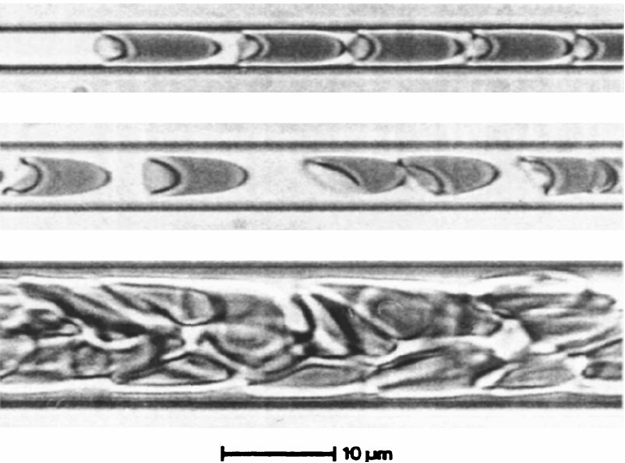
\includegraphics[width = 1.5in]{Rbcflow.PNG} \csy{Pozrikidis, 2006}\end{center}

  	\begin{center} Cardiac mechanics 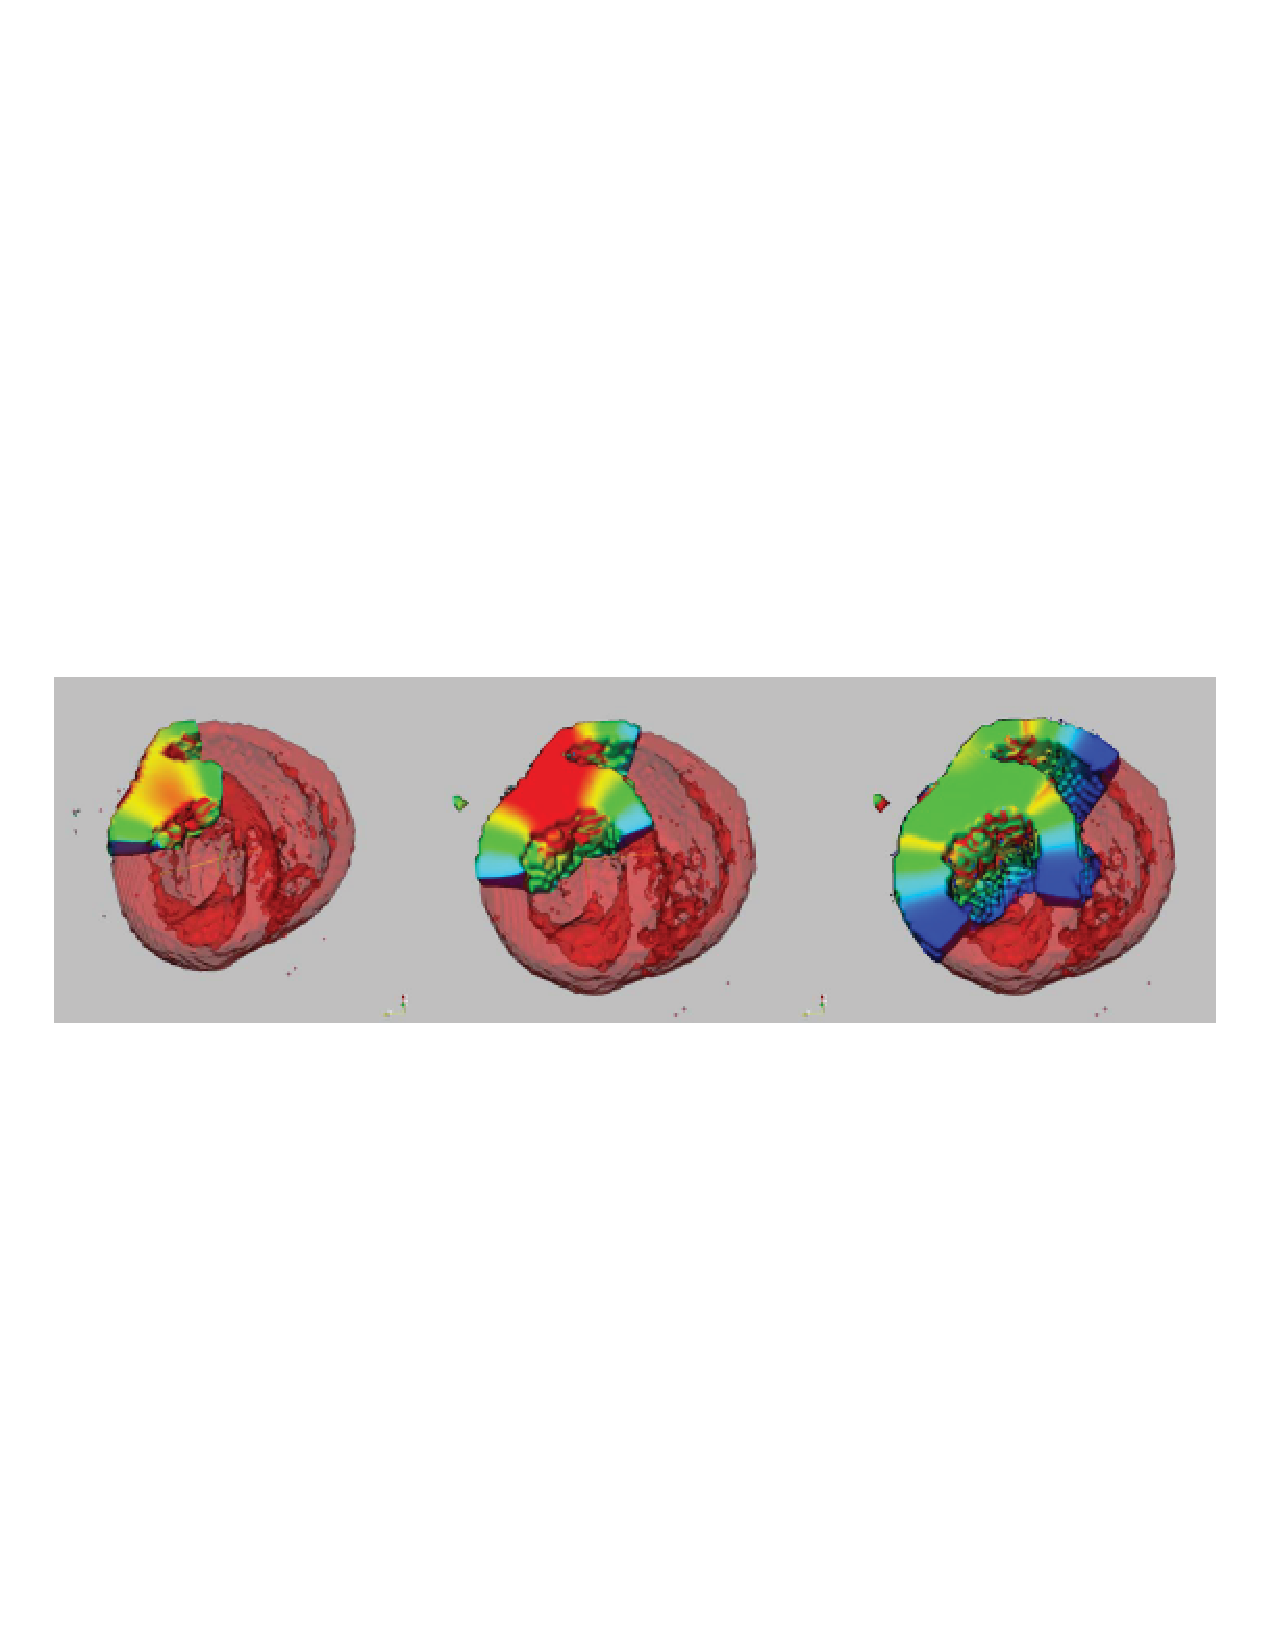
\includegraphics[width = 2in]{heart} \csy{Adavani-Biros,2008}\end{center}

\end{column}
\begin{column}{.5\textwidth}
    \begin{center}Design of MEMS 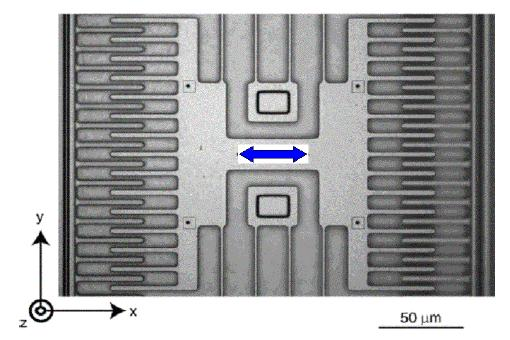
\includegraphics[width = 1.6in]{resonator.jpg} \csy{White's group (MIT)}\end{center}
    
\begin{block}{Common challenges}
\begin{itemize}
 \item Moving geometries
 \item Multi-scale phenomena
 \item
 \item
\end{itemize}
\end{block}

\end{column}
\end{columns}
\end{frame}

\begin{frame}
\frametitle{Introduction }
\framesubtitle{Related Work}
\begin{block}{Sequential}

\end{block}

\begin{block}{Parallel}

\end{block}
\end{frame}

